% Created 2014-12-27 Sat 20:34
\documentclass[11pt]{article}
\usepackage[utf8]{inputenc}
\usepackage[T1]{fontenc}
\usepackage{fixltx2e}
\usepackage{graphicx}
\usepackage{longtable}
\usepackage{float}
\usepackage{wrapfig}
\usepackage[normalem]{ulem}
\usepackage{textcomp}
\usepackage{marvosym}
\usepackage{wasysym}
\usepackage{latexsym}
\usepackage{amssymb}
\usepackage{amstext}
\usepackage{hyperref}
\tolerance=1000
\author{Giulio Bottazzi}
\date{\today}
\title{gbutils: cygwin installation}
\hypersetup{
  pdfkeywords={},
  pdfsubject={},
  pdfcreator={Emacs 23.4.1 (Org mode 8.0.6)}}
\begin{document}

\maketitle
\tableofcontents



\section{Introduction}
\label{sec-1}

The present document provides a short description of how to install
the gbutils package inside a \href{https://www.cygwin.com/}{Cygwin} environment.

From its website "Cygwin is a large collection of GNU and Open Source
tools which provide functionality similar to a Linux distribution on
Windows". The Cygwin DLL currently works with all recent, commercially
released x86 32 bit and 64 bit versions of Windows, starting with
Windows XP SP3.
\section{Install Cygwin}
\label{sec-2}

You can skip this part if you use Cygwin already. Otherwise follow the
instructions.

From the \href{https://www.cygwin.com/}{Cygwin} website download the installation program on the
windows machine. There is both a 32 bit and a 64 bit flavor. Launch
the executable. It will require to set a few parameters, but I usually
accept the default setting. Then you are presented with a page that
ask you to select extra packages for installation, similar to the
picture below.


\begin{figure}[htb]
\centering
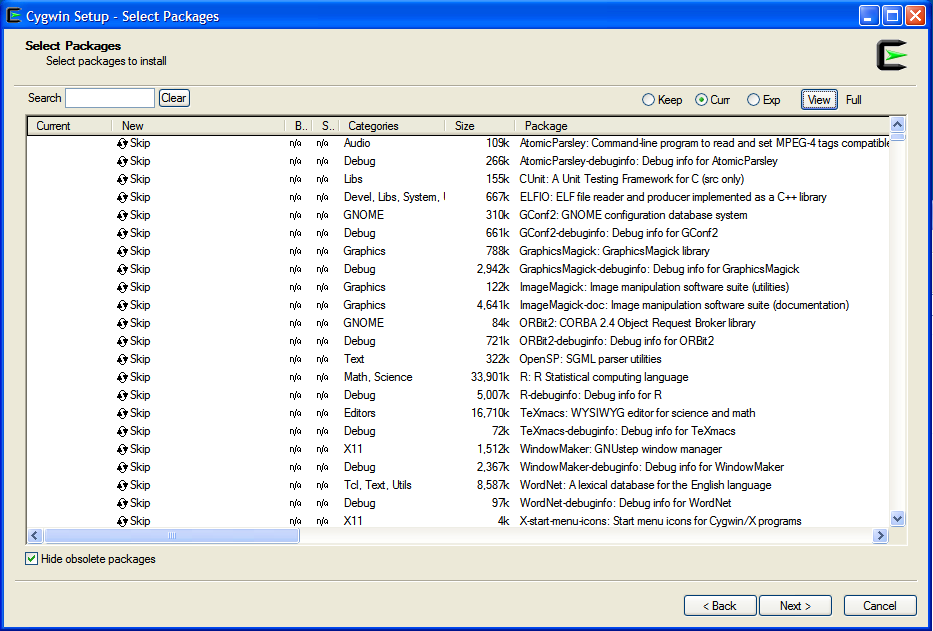
\includegraphics[width=.9\linewidth]{cygwin_install.png}
\caption{Cygwin packages selection window.}
\end{figure}

From this window select the packages (by clicking on the "circular
arrows" symbol on the left) \texttt{gsl} and \texttt{gsl-devel}. Moreover check that
the packages \texttt{crypt} and \texttt{make} are selected. They should be already,
but you never know. If you plan to install the libmatheval support
(highly recommended) install also \texttt{flex}, \texttt{guile}, \texttt{guile-devel},
\texttt{libgmp} and \texttt{libgmp-devel}.
\section{Install GNU matheval library}
\label{sec-3}

Download the last package from the \href{https://www.gnu.org/software/libmatheval/}{libmatheval website}. It should have
extension \texttt{.tar.gz}. Move the package in \texttt{c:\textbackslash{}cigwin\textbackslash{}usrl\textbackslash{}local} and
launch the \texttt{Cygwin desktop} (an icon should have been created in your
Desktop). Inside the shell move to \texttt{/usr/local/} and unpack the source
code

\begin{verbatim}
tar xvzf libmatheval-{version}.tar.gz
\end{verbatim}

move inside the source directory

\begin{verbatim}
cd libmatheval-{version}
\end{verbatim}

run the configure script specifying the prefix \texttt{/usr}

\begin{verbatim}
./configure --prefix=/usr
\end{verbatim}

then build the files

\begin{verbatim}
make
\end{verbatim}

and install them

\begin{verbatim}
make install
\end{verbatim}

If more detailed instructions are necessary, see the file \texttt{INSTALL} in
the source directory (you can use the command \verb~less INSTALL~).

\section{Install gbutils}
\label{sec-4}

From the \href{ftp://cafed.sssup.it/packages/}{cafed repository} download the last \texttt{tar.gz} package and move
it in the \texttt{/usr/local/} directory. In the \texttt{Cygwin desktop} unpack the
package:
\begin{verbatim}
tar xvzf gbutils-{version}.tar.gz
\end{verbatim}
move inside the source directory
\begin{verbatim}
cd gbutils-{version}
\end{verbatim}
run the configure script
\begin{verbatim}
./configure
\end{verbatim}
then build the files
\begin{verbatim}
make
\end{verbatim}
and install them
\begin{verbatim}
make install
\end{verbatim}

If more detailed instructions are necessary, see the file \texttt{INSTALL} in
the source directory (you can use the command \verb~less INSTALL~).

This is the END, enjoy your gbutils :-)
% Emacs 23.4.1 (Org mode 8.0.6)
\end{document}